\documentclass[a4paper, 15pt]{article}
\usepackage[left=0.85in, right=0.85in, top=0.5in, bottom=0.95in]{geometry}
\usepackage[T1]{fontenc}
\usepackage[utf8]{inputenc}
\usepackage[italian]{babel}
\usepackage[none]{hyphenat} % no sillabazione 
\usepackage{multicol} %testo su più colonne
\usepackage{enumitem}
\usepackage{mdwlist} %suspend enumerate \suspend{} \resume{}
\usepackage{lipsum} %testo random per verifica \lipsum
\usepackage{graphicx, nicefrac}
\usepackage{wrapfig2}
\usepackage{amsmath}
\usepackage{mathtools}
\usepackage{amssymb}
\usepackage{amsthm} %teoremi e dimostrazioni e definizioni
\usepackage{cases}
\usepackage{gensymb} %simboli come ° = \degree  etc etc
\usepackage{cancel} %permette di fare semplificazioni utilizzando il comando \cancel{expression}
\usepackage{subcaption}
\usepackage{hyperref}
\hypersetup{
	colorlinks=true,
	linkcolor=blue,    
	urlcolor=blue,
	%pdfpagemode=FullScreen, %il pdf generato non si avvia a schermo intero
}
\urlstyle{same}
\usepackage{changepage}
\usepackage{lastpage, epstopdf}
\usepackage{fancyhdr}
\usepackage{tcolorbox}
%\usepackage{background} %non utilizza lo sfondo con "draft"
\usepackage{color} % testo colorato \textcolor{'ColorCode'}{'testo'}
\usepackage{setspace} % in questo modo posso settare lo spoazio dell'indice \begin{spacing}{0.95}	
\usepackage{changepage}
\usepackage{lastpage, epstopdf}
\usepackage{fancyhdr}
\usepackage{tcolorbox}
%\usepackage{background}
%%%%%%%%%%%%%%%%%%%%%%%%%%%%%%%%%%%%%%%%%%%% AMBIENTE TIKZ 
\usepackage{tikz} %disegni e mappe
\usetikzlibrary{patterns}
\usepackage{pgfplots}
\pgfplotsset{compat=1.15}
\usepackage{mathrsfs}
\usetikzlibrary{arrows,decorations.markings,arrows.meta, decorations.text}
\usepackage{circuitikz}
\tikzset{immagine/.style={%
			above right, inner sep=0pt, outer sep=0pt},
		testo/.style={fill=white, align=center,
			fill opacity=0.6, text opacity=1, below,
			font=\sffamily\bfseries\footnotesize}}
\raggedbottom
\setlength{\parindent}{0pt}
%%%%%%%%%%%%%%%%%%%%%%%%%%%%%%%%%%%%%%%%%%%% SIUNITX 
\usepackage{siunitx}

%========TEOREMI========%
\newtheorem*{thm}{Teorema}
\newtheorem*{en}{Enunciato}
\newtheorem*{definizione}{Definizione}
\newtheorem*{cor}{Corollario}
%========OPERATORI&COMANDI========%
\DeclareMathOperator{\rk}{rk}
\DeclareMathOperator{\im}{Im}
\DeclareUnicodeCharacter{20AC}{\EUR}
\usepackage{pifont}
\newcommand{\cmark}{\ding{51}}
\newcommand{\xmark}{\ding{55}}
\newcommand{\compresslist}{ % Define a command to reduce spacing within itemize/enumerate environments, this is used right after \begin{itemize} or \begin{enumerate}
				\setlength{\itemsep}{1pt}
				\setlength{\parskip}{0pt}
				\setlength{\parsep}{0pt}
			}
\newcommand{\ra}[1]{\renewcommand{\arraystretch}{#1}} %stretcho le tabelle			
\renewcommand{\arraystretch}{2.5} % Da copiaincollare prima di ambienti array per ampliarli un po'
\setlength{\jot}{10pt} % affecting the line spacing in the environment SPLIT
			
\title{8. MISURE DI SPOSTAMENTO E VELOCITÀ}
%%\author{A.M.}
\date{}

\begin{document}

	\maketitle
	\setcounterpageref{secnumdepth}{0}	
	\tableofcontents 
	\newpage
	
\begin{adjustwidth}{2in}{}
	Per effettuare le misure di spostamento  e velocità possono essere adottati due sistemi di misura 
	\begin{itemize}
		\item \textbf{Con riferimento fisso}: fornisce la variabile cinematica nelle variabili di riferimento fisse. 
		
		La misura si esprime rispetto ad un sistema solidale col fisso.
		
		Si usano potenziometri, LVDT, encoder, laser a triangolazione.
		\item \textbf{Senza riferimento fisso}: la misura si esprime secondo assi solidali al sensore stesso. 
		
		Si usano accelerometri, sensori inerziali, non trattati in questo corso. 
	\end{itemize}
\begin{center}
	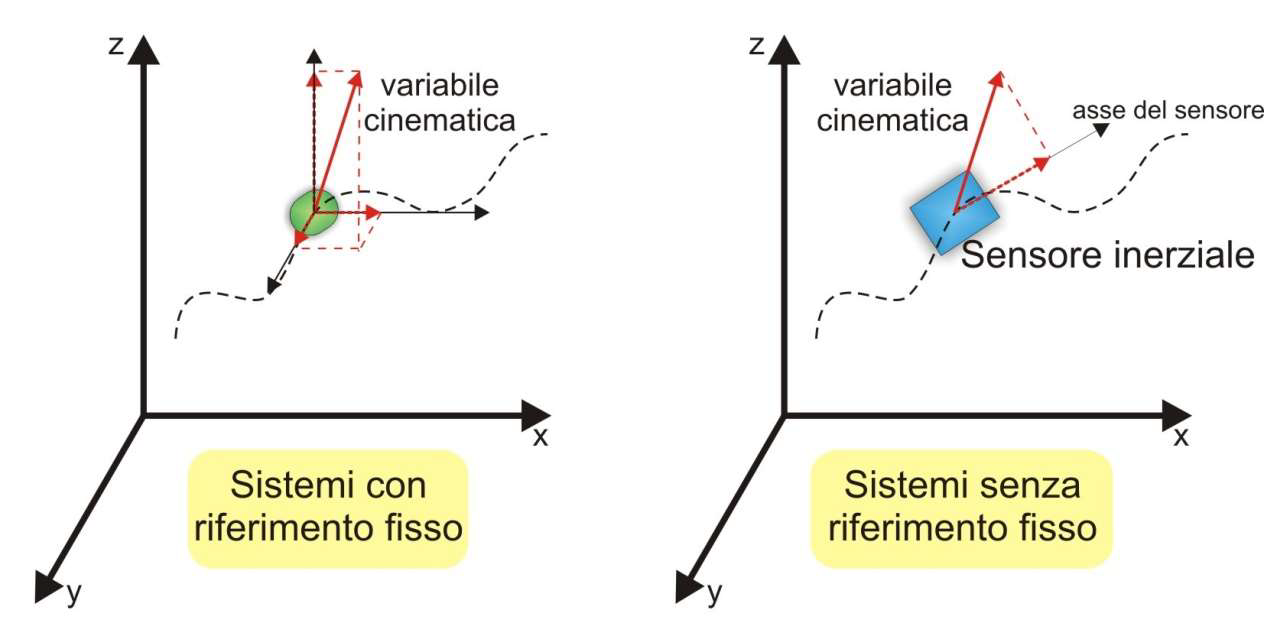
\includegraphics[width=0.7\linewidth]{immagini/sistemi}
\end{center}
\end{adjustwidth}


\section{Misure di Spostamento}
\subsection{Potenziometro}
\begin{adjustwidth}{2in}{}
	Il potenziometro è un sistema di misura utilizzato per rilevare spostamento lineari e angolari. 
	
	In ingresso prende una lunghezza ed in uscita fornisce una resistenza. 	
	\begin{figure}[H]
		\centering
		\begin{tikzpicture}[>=latex]
		%\draw [help lines] (0,0) grid (4,4);
		\draw (0,0) rectangle (2,1);
		\draw [->] (-1,0.5) -- (0,0.5) node [pos=0, sloped, above] {$\Delta\theta, \Delta x$};
		\draw [->] (2,0.5) -- (3,0.5) node [pos=0.5, sloped, above] {$\Delta R$};
	\end{tikzpicture}
	\end{figure}
	 È realizzato mediante un filo di materiale conduttivo avvolto introno ad un supporto rigido.
	 \begin{center}
	 	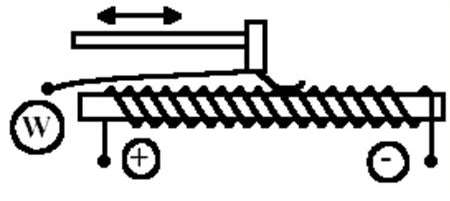
\includegraphics[width=0.4\linewidth]{immagini/potenz}
	 \end{center}	 
\end{adjustwidth}
\newpage			
\subsubsection{Potenziometro Ideale}
\begin{adjustwidth}{2in}{}
	Le equazioni de potenziometro reale si ottengono considerando un voltmetro ideale $E_0$ a $R_s\rightarrow\infty$, nello strumento terminale non scorre correte, in questo modo si ottiene una perfetta linearità. 
	
	Nella realtà un minimo di corrente scorre, altrimenti non si misurerebbe alcuna resistenza.
	\begin{center}
		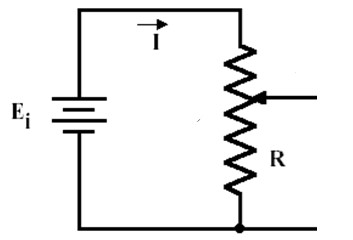
\includegraphics[width=0.4\linewidth]{immagini/potenz1}
	\end{center}
	La resistenza del potenziometro varia da 
	\[R_P = [0;R_P]\]
	La resistenza misurata varia da 
	\[R = [0;R]\]
	Alimentando il circuito con $E_I$ scorre corrente, si misura perciò
	\[E_0 = [0;E_i]\]
	Perciò
	\[E_0 = IR \qquad E_i = IR_p\]
	\[R = \rho{l\over S} \qquad R_P = \rho{l_p\over S}\]
	In cui $l = x$ ed $l_P = L$ sono rispettivamente la lunghezza del filo fino al palpatore ( la distanza percorsa dal palpatore) e la lunghezza del filo del potenziometro (la distanza massima del palpatore)
	\[E_0 = E_i{R\over R_p} = E_i{l\over l_p} = E_i{x\over L}\]
	La \textbf{sensibilità} diviene pari a
	\[S = {E_i\over L}\]
	Funzione della tensione di alimentazione del potenziometro, facendo pur sempre attenzione all'autoriscaldamento. 
	
	La resistenza del potenziometro non può essere troppo piccola altrimenti si avrebbe un'elevata dispersione per effetto Joule 
	\[P_{\max}= {E_i^2\over R_p}\]
	La \textbf{risoluzione} dei potenziometri del tipo a filo avvolto è pari a ${L\over n}$ dove $L$ è la distanza massima misurabile e $n$ è il numero totale degli avvolgimenti. 
	\begin{center}
		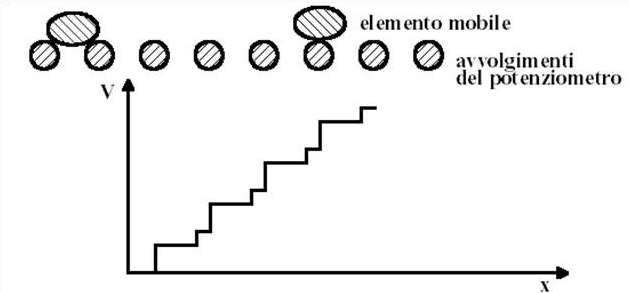
\includegraphics[width=0.4\linewidth]{immagini/potenz2}
	\end{center}
	È necessario avvicinare le spire per ottenere una maggiore risoluzione, un'alternativa a questo problema è data dalla plastica conduttiva.	
\end{adjustwidth}
\subsubsection{Potenziometro Reale}
\begin{adjustwidth}{2in}{}
	Il potenziometro reale si differenzia da quello ideale per lo strumento terminale: infatti ora questo sarà percorso da corrente $R_s\nrightarrow\infty$; la corrente che prima scorreva soltanto sul potenziometro ora si splitta anche sullo strumento terminale. 
	\begin{center}
		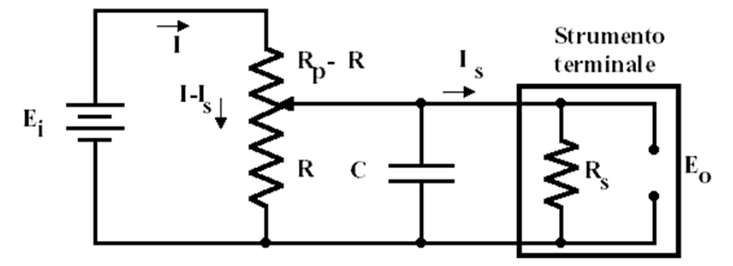
\includegraphics[width=0.4\linewidth]{immagini/potenz3}
	\end{center}	
	Per trovare le equazioni del potenziometro reale si sfruttano le equazioni delle maglie. 
	
	\[E_0 = I_sR_s\qquad E_0 = (I-I_s)R \qquad E_0 = E_i - I(R_p-R)\]
	
	\[I_s = {E_0 \over R_s}\]
	\[E_0 = IR - I_sR \qquad E_0 = IR - {E_0\over R_s}R\]
	\[I = E_0\left({1\over R}+{1\over R_s}\right)\]
	\[E_0 = E_i - E_0\left({1\over R}+{1\over R_s}\right)(R_p-R)\]
	\[E_i = E_0\left(1+\left({1\over R}+{1\over R_s}\right)(R_p-R)\right)\]
	\[E_i = E_0\left(1+\left(\dfrac{R+R_s}{RR_s}\right)(R_p-R)\right)\]
	\[E_i = E_0\left(\dfrac{RR_s + (R+R_s)(R_p-R)}{RR_s}\right)\]
	Allora
	\[RR_sE_i = E_0(RR_s RR_p - R^2 + R_sR_p-RR_s)\]
	\[E_0 = E_i\left(\dfrac{RR_s}{RR_p-R^2+R_sR_p}\right)\]
	Dividendo numeratore e denominatore per $R_p^2$ si ottiene 
	\[E_0 = \left(\dfrac{\nicefrac{R_s}{R_p}}{\nicefrac{R_s}{R_p} +\nicefrac{R}{R_p} + (\nicefrac{R}{R_p})^2}\right)\cdot{R\over R_p}E_i\]
	Ci si vuole ricondurre ad un'equazione simile a quella trovata per il potenziometro ideale, si introduce allora il fattore di carico o di non linearità
	\[\eta = \dfrac{\nicefrac{R}{R_p} - (\nicefrac{R}{R_p})^2}{\nicefrac{R_s}{R_p} + \nicefrac{R}{R_p} - (\nicefrac{R}{R_p})^2 }\]
	Per cui
	\[E_0 = (1-\eta){R\over R_p}E_i\]
	Da cosa dipende il fattore di carico? dal rapporto $\nicefrac{R}{R_p}$, quindi da dove si sta effettuando la misura. 
	
	Inoltre, similmente all'errore di inserzione per le misure di tensione, se
	\[\eta\rightarrow0\Rightarrow{R_s\over R_p}\rightarrow\infty \Rightarrow R_s\gg R_p\]
	E allora si ricade nell'idealità. 
	
	$\eta$ si configura così come un parametro che indica quanto è distante lo strumento dall'idealità.
	\begin{center}
		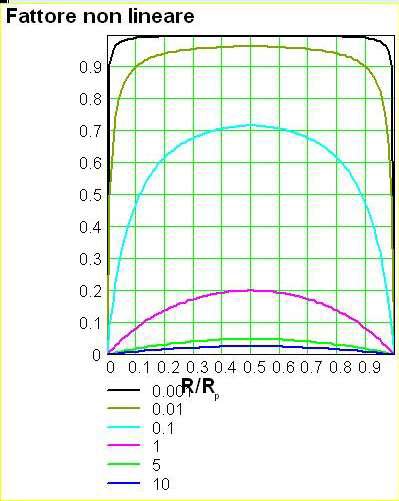
\includegraphics[width=0.6\linewidth]{immagini/potenz4}
	\end{center}
	Dal grafico del fattore di carico si vede che, se
	\begin{itemize}
		\item ${R_s\over R_p} = 10$ e quindi c'è un fattore 10 tra l'una e l'altra, $\eta$ è molto basso
		\item ${R_s\over R_p} = 0.1$ $\eta$ diviene elevatissimo, induce un errore variabile a parabola che nel suo massimo può arrivare al 70\% del valore misurato
		\item ${R_s\over R_p} = 0.001$ $\eta$ raggiunge quasi l'unità, l'uscita misurata è nulla: l'insieme potenziometro-strumento non hanno le impedenze corrette.
	\end{itemize}
	Impossibile non notare come il punto più critico nella misura di un potenziometro sia quello centrale.
	\begin{center}
	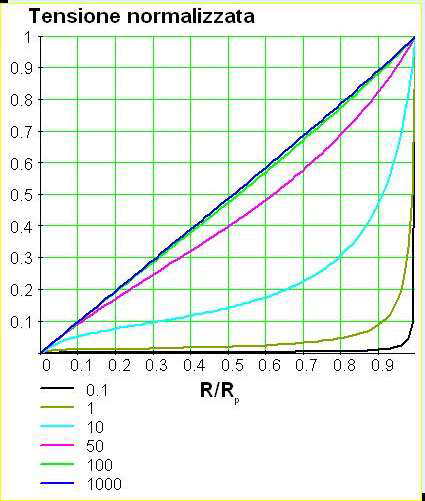
\includegraphics[width=0.6\linewidth]{immagini/potenz5}
	\end{center}
	Dal grafico della tensione normalizzata si nota invece che, per $\eta\rightarrow0$ si ottiene la bisettrice, e come $\nicefrac{R_s}{R_p}\downarrow$ la curva diventi fortemente non lineare, dallo 0 cresce molto velocemente al massimo.  
\newpage
	\textcolor{red}{\textbf{PROBLEMA}}\\
	Come misurare la tensione in uscita da un sensore di elevata impedenza? \\
	
	\textcolor{green}{\textbf{SOLUZIONE}}\\
	Si inserisce tra il trasduttore e lo strumento terminale un amplificatore operazionale in configurazione buffer, in questo modo si sostituisce ad $R_s$ la resistenza dell'amplificatore $10^6\div10^9~\Omega$
	\begin{center}
		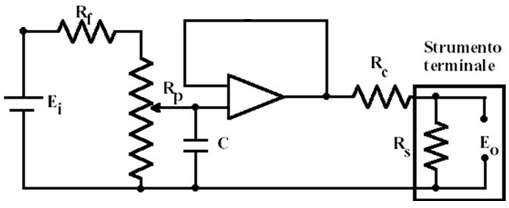
\includegraphics[width=0.5\linewidth]{immagini/potenz6}
	\end{center}
	
	\textcolor{red}{\textbf{PROBLEMA}}\\
	Necessaria una misura della resistenza escludendo il contributo dei cavi di collegamento. \\
	
	\textcolor{green}{\textbf{SOLUZIONE}}\\
	Attraverso un multimetro che lo permetta, si esegue una misura diretta con 4 fili, si ottiene cosi direttamente la misure che interessa. 
	
	La caduta di potenziale $E_C$ che si manifesta ai connettori A e D non ha effetto nella determinazione della caduta di potenziale ai capi del potenziometro e l'impedenza del voltmetro è tale da rendere trascurabile la caduta di potenziale che
	si ha ai connettori B e C.
	\begin{center}
		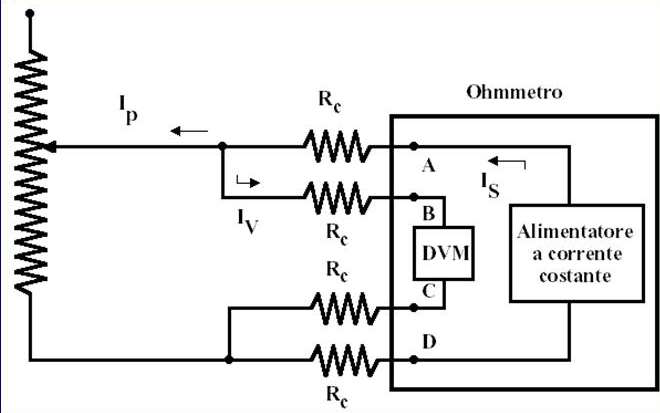
\includegraphics[width=0.5\linewidth]{immagini/potenz7}
	\end{center}
\end{adjustwidth}
\newpage
\subsection{LVDT}
\begin{adjustwidth}{2in}{}
		Il trasformatore differenziale è utilizzato per la misura di piccoli spostamenti sia lineari che angolari. 
\begin{figure}[H]
	\centering
	\begin{tikzpicture}[>=latex]
	%\draw [help lines] (0,0) grid (4,4);
	\draw (0,0) rectangle (2,1);
	\draw [->] (-1,0.5) -- (0,0.5) node [pos=0, sloped, above] {$\Delta\theta, \Delta x$};
	\draw [->] (2,0.5) -- (3,0.5) node [pos=0.5, sloped, above] {$\Delta L$};
\end{tikzpicture}
\end{figure}
	Dove $L$ è l'induttanza. \newline 
	
	È costituito da un cilindro cavo di materiale metallico ad alta permeabilità magnetica al cui interno può scorrere senza contatto un nucleo ferromagnetico, al di fuori del cilindro vi sono avvolte 3 bobine simmetriche di filo conduttivo. 
\begin{center}
	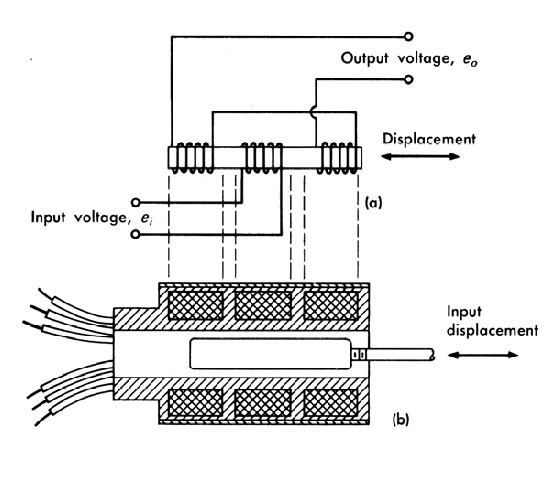
\includegraphics[width=0.5\linewidth]{immagini/LVDT}
\end{center}	
	L'avvolgimento primario è il centrale, mentre gli avvolgimenti laterali sono i secondari. 
		
	In uscita si misura la differenza di induttanza tra i due secondari, facendo scorrere il nucleo all'interno del cilindro si perde la simmetria e si misura una tensione al secondario proporzionale al primario attraverso le leggi della la mutua induttanza. 	
	\begin{center}
		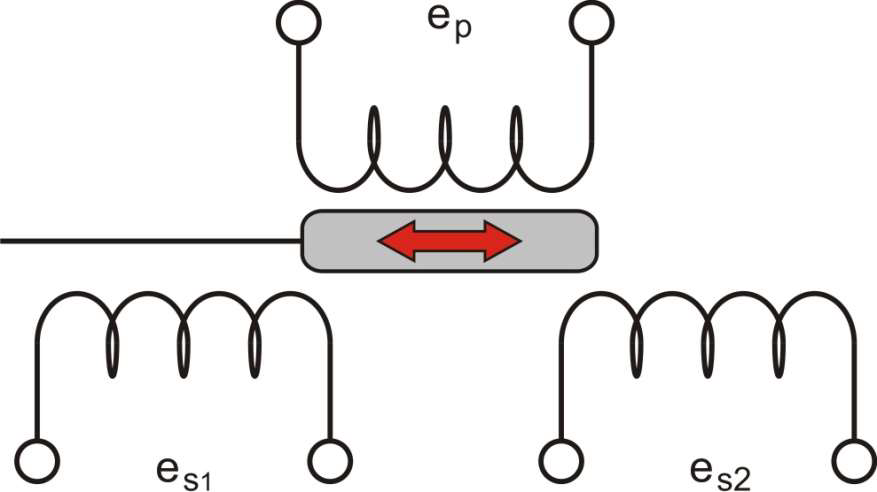
\includegraphics[width=0.5\linewidth]{immagini/LVDT1}
	\end{center}
	L’avvolgimento primario è alimentato da una tensione alternata di opportuna
	frequenza mentre gli avvolgimenti secondari sono avvolti in senso discorde e ricevono, per
	induzione elettromagnetica dal primario, le tensioni $e_{s1}$ ed $e_{s2}$, secondo lo schema 
	\begin{center}
		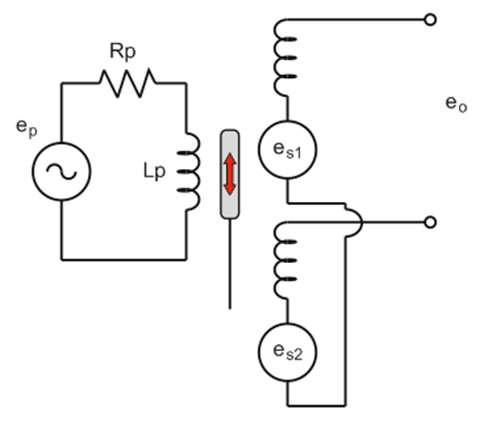
\includegraphics[width=0.5\linewidth]{immagini/LVDT2}
	\end{center}
	\newpage
	L'induttanza è pari a 
	\[L = \mu FN^2\]
	E le mutue induttanze sono
	\[M_1 = \sqrt{L_1\cdot L_p} \qquad M_2 = \sqrt{L_2\cdot L_p}\]
	Ricordando che 
	\[i_pR_p + L_p{di_p\over dt}-e_p = 0 \]
	Si individua allora 
	\[e_0 = e_{s1} - e_{s2} = (M_1-M_2){di_p\over dt}\]
	Quando il nucleo è centrato $e_0=0$ non si misura alcuna tensione, sarà lo spostamento del nucleo ad agisce sui coefficienti di mutua induzione, modificandoli e portando ad una misurazione di una tensione alternata alla frequenza del segnale in ingresso.
	\begin{center}
		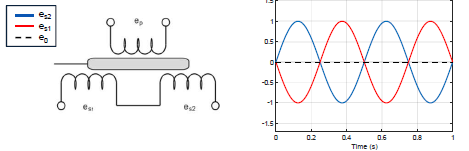
\includegraphics[width=0.5\linewidth]{immagini/screenshot001}
	\end{center}
	\begin{itemize}
		\item \[e_{s2}>e_{s1}\]
		La tensione in uscita $e_0$ è sinusoidale e ha fase opposta alla tensione in ingresso (-).
		\begin{center}
			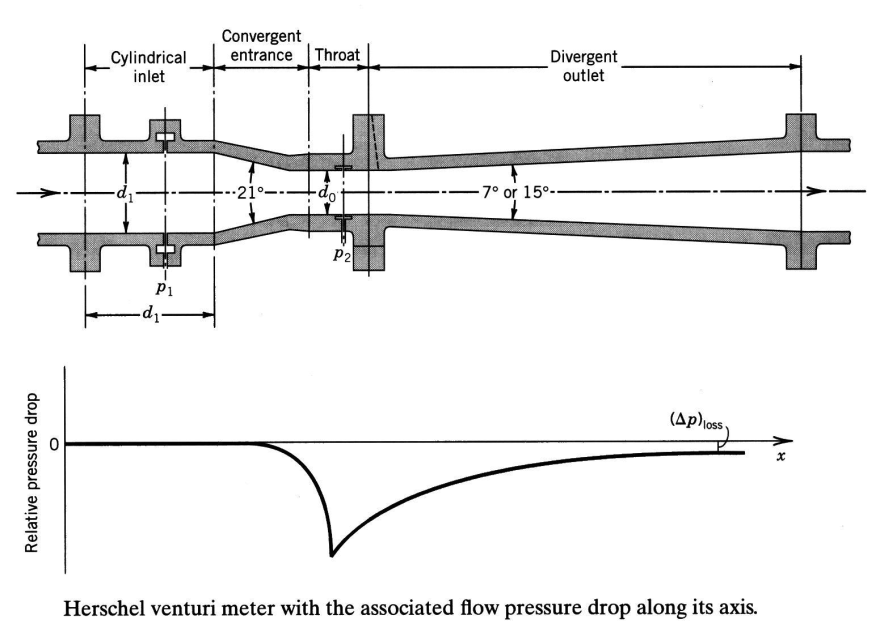
\includegraphics[width=0.5\linewidth]{immagini/screenshot002}
		\end{center}
		Lo spostamento è verso destra $\rightarrow$.
		
		\item \[e_{s1}>e_{s2}\]
		La tensione in uscita è sinusoidale e ha la stessa fase della tensione in ingresso (+).
		\begin{center}
			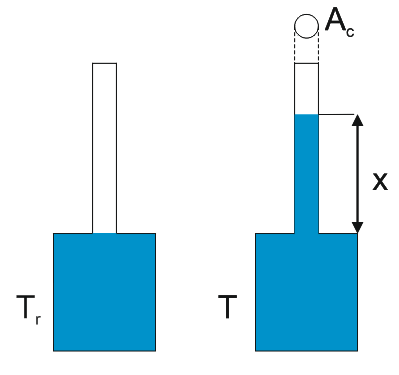
\includegraphics[width=0.5\linewidth]{immagini/screenshot003}
		\end{center}		
		Lo spostamento è verso sinistra $\leftarrow$. 		
	\end{itemize}
	In questo modo dalla tensione in uscita $e_0$ si può determinare sia l'ampiezza dello spostamento (dall'ampiezza del segnale), sia il verso dello spostamento (dalla fase del segnale), ovviamente per ottenere il verso dalla fase sarà necessario un circuito elettrico detto "discriminatore di fase".\newline 
	
	\begin{itemize}[label={\textcolor{red}{\xmark}}]
	\item Nell'LVDT è necessario fare molta \textcolor{red}{attenzione} al \textbf{campo di misura}, questo infatti è compreso tra i \qtylist{5;10}{\centi\metre}
	\begin{center}
		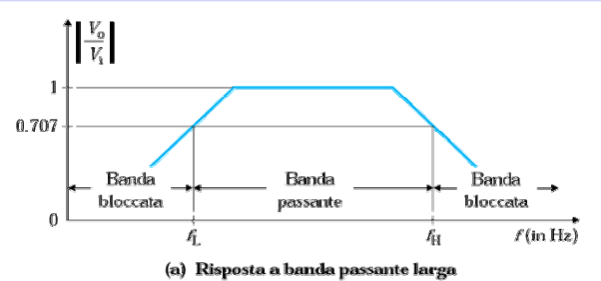
\includegraphics[width=0.5\linewidth]{immagini/screenshot004}
	\end{center}
	Ed è limitato dalla quantità di spire/avvolgimenti che si possono fisicamente realizzare: lo strumento va in saturazione perché finisco le spire, per cui oltre alla zona di linearità la sensibilità crolla inevitabilmente a 0.  
	
	\item È possibile utilizzare l'LVDT per effettuare \textbf{misure dinamiche}?
	
	Sono se il valore della frequenza portante è almeno 10 volte superiore alla frequenza dell'armonica ritenuta ancora significativa nella rappresentazione del fenomeno fisico (principio di Shannon): la frequenza di spostamento dev'essere minore di quella di alimentazione, altrimenti non diviene possibile visualizzare nè misurare alcuna sinusoide.  
	
	\item Tra i fenomeni fisici che limitano la tensioni di alimentazione applicabile di trovano l'effetto Joule e l'aumento della non linearità nell'accoppiamento magnetico.
	
	\item Il disegno simmetrico del trasduttore rende il trasformatore differenziale
	particolarmente immune da effetti indotti da variazioni statiche e quasistatiche
	della temperatura, tuttavia se dovesse variare la temperatura varierebbe giocoforza anche la resistenza elettrica degli avvolgimenti elettrici del primario, e quindi anche l'intensità di corrente che scorre negli avvolgimenti, portando quindi ad una variazione della sensibilità del trasduttore.  
	
	\item Anche in presenza di un perfetto allineamento tra i vari elementi costituenti, il
	trasformatore differenziale fornisce in uscita un segnale diverso da zero a
	causa delle capacità parassite presenti tra gli avvolgimenti.
	\end{itemize}
\end{adjustwidth}
%\newpage
\subsection{Encoder}
\begin{adjustwidth}{2in}{}
	L'encoder converte uno spostamento in un segnale digitale e permette la misurazione di una variazione angolare. 
	\begin{center}
		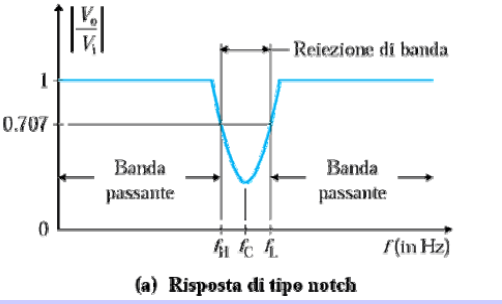
\includegraphics[width=0.5\linewidth]{immagini/screenshot005}
	\end{center}
	Possono essere 
	\begin{itemize}
		\item \textbf{Incrementali}, se misurano una distanza rispetto ad una posizione iniziale 
		\item \textbf{Assoluti}, se misurano una distanza assoluta rispetto ad un punto fisso.
	\end{itemize}
	Nella realizzazione invece si possono dividere in 
	\begin{itemize}
		\item \textbf{Encoder ottico}
		\begin{center}
			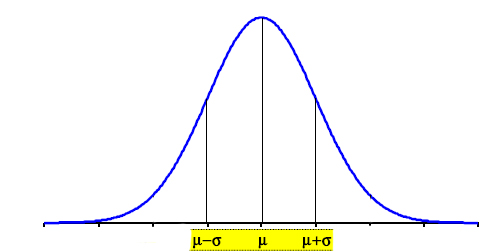
\includegraphics[width=0.5\linewidth]{immagini/screenshot006}
		\end{center}
		Un disco composto da zone trasparenti ed elementi scuri è posto solidalmente ad un albero posto in rotazione. 
		
		Un fotorilevatore assorbe ciò che un emettitore produce attraverso le zone trasparenti del disco.
		
		L'uscita di questo segnale è a gradino.
		
		\item \textbf{Encoder a strisciamento}
		\begin{center}
			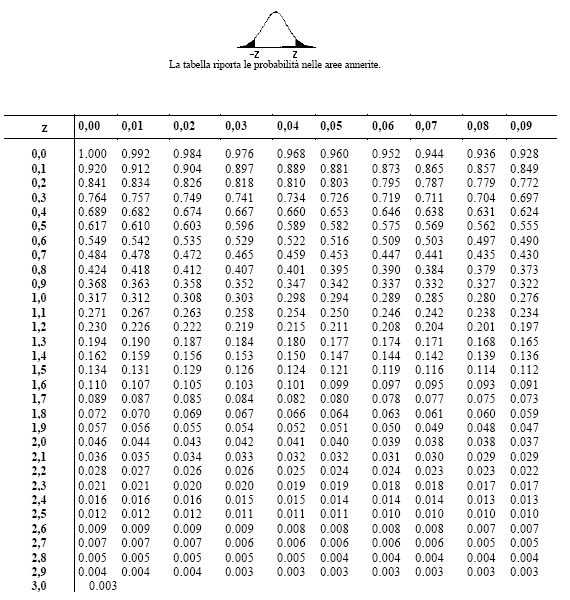
\includegraphics[width=0.5\linewidth]{immagini/screenshot007}
		\end{center}
		Il disco frammentato è fisso all'albero, si esegue così una misura di torsione tra due contatti striscianti.
		
		L'uscita di questo segnale è a gradino.
\newpage		
		\item \textbf{Encoder magnetico}
		 \begin{center}
		 	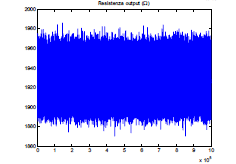
\includegraphics[width=0.5\linewidth]{immagini/screenshot008}
		 \end{center}
		 In questa applicazione, tra ingresso e uscita c'è un trasformatore, l'uscita di questo segnale è grossomodo sinusoidale
	\end{itemize}
	In ogni caso il segnale in uscita sarà un segnale digitale che varia tra due stati. 
\end{adjustwidth}
%\newpage
\subsubsection{Encoder Incrementale}
\begin{adjustwidth}{2in}{}
	L'encoder incrementale misura la rotazione o lo spostamento lineare in funzione del numero di fronti di salita o discesa acquisiti. 
	\begin{center}
		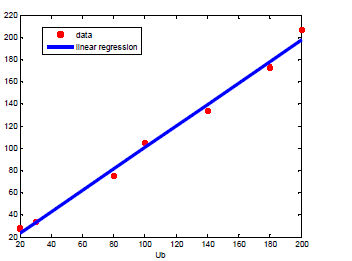
\includegraphics[width=0.5\linewidth]{immagini/screenshot009}
		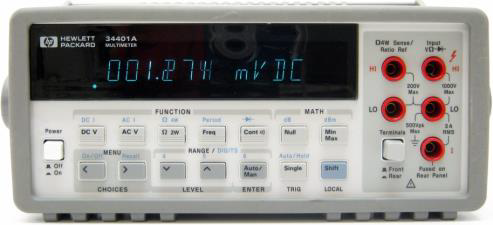
\includegraphics[width=0.5\linewidth]{immagini/screenshot010}
		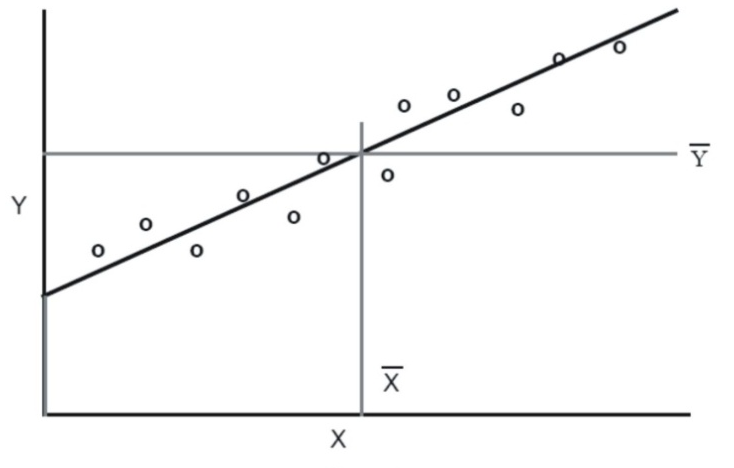
\includegraphics[width=0.5\linewidth]{immagini/screenshot011}
	\end{center}
	Per individuare la misura della rotazione basterà così contare i fronti d'onda individuati dal sensore. 
	
	Gli aspetti critici di questa prima realizzazione risiedono nel fatto che
	\begin{itemize}[label={\textcolor{red}{\xmark}}]
		\item La risoluzione dipende dall'ampiezza degli spazi
		\item La direzione di rotazione non è un output fornito.
	\end{itemize} 
	\begin{itemize}[label={\textcolor{green}{\cmark}}]
		\item Il problema del verso dello spostamento viene risolto introducendo un secondo elemento/disco generatore di segnale, in questo modo i segnali risulteranno sfasati di 1/4.
		\begin{center}
			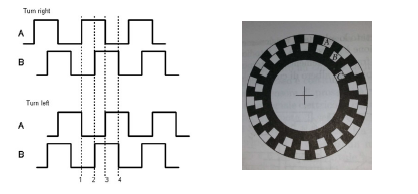
\includegraphics[width=0.5\linewidth]{immagini/screenshot012}
		\end{center}
		\item Il problema della risoluzione viene invece risolto dalla specifica codifica dell'encoder, questo infatti può avere codifica 1x, 2x, 4x in funzione del numero di fronti d'onda presi in considerazione per il calcolo dello spostamento.
		\begin{center}
			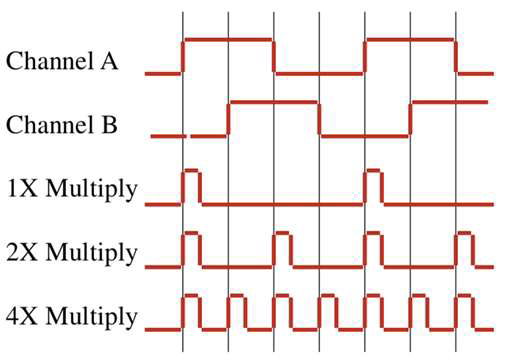
\includegraphics[width=0.5\linewidth]{immagini/screenshot013}
		\end{center}
		Se inoltre si realizza un'ulteriore fessura nel disco e si aggiunge un'altra coppia di led e fotodiodo relativa a tale fessura, può essere realizzato anche un segnale che fornisce il periodo di rotazione.		
	\end{itemize}
\end{adjustwidth}
%\newpage
\subsubsection{Encoder Assoluto}
\begin{adjustwidth}{2in}{}
	Negli encoder assoluti si ha una determinazione della posizione assoluta assunta dall'organo mobile indipendentemente dalla condizione iniziale di riferimento: la posizione si "ricorda" perché è l'ultima posizione assunta dallo strumento. \newline
	
	 Per far ciò essi necessitano un altro tipo di corona e di una “schiera” di rivelatori in parallelo.
	 \begin{center}
	 	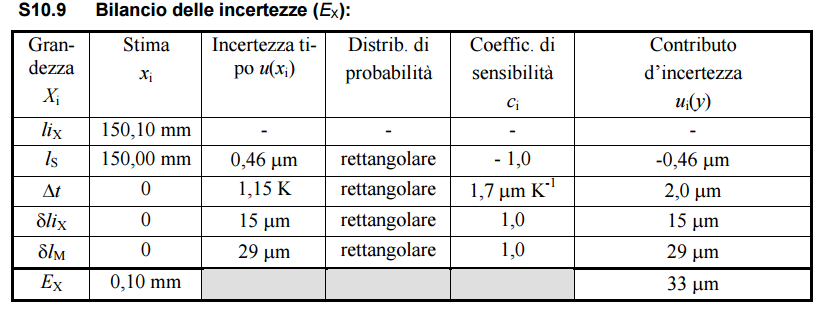
\includegraphics[width=0.3\linewidth]{immagini/screenshot014}
	 \end{center}
	 In questo modo ogni traccia rappresenta direttamente il valore del rispettivo bit ed è la combinazione dei bit in codice binario, a fornire la misura finale.
	 \begin{figure}[H]
	 	\centering
	 	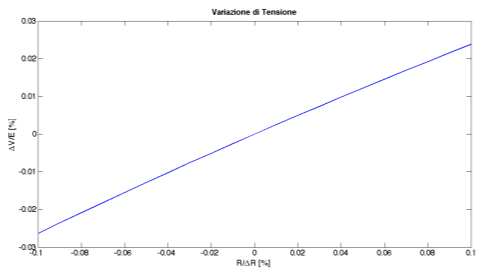
\includegraphics[width=0.5\linewidth]{immagini/screenshot015}
	 	\caption{Encoder a 4 bit}
	 	\label{fig:screenshot015}
	 \end{figure}
	 \begin{center}
	 	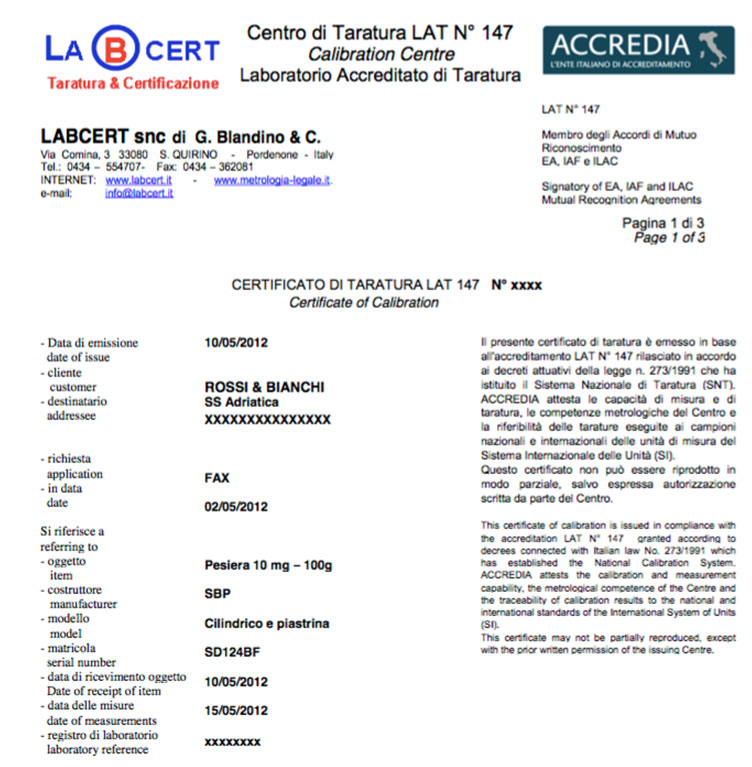
\includegraphics[width=0.7\linewidth]{immagini/screenshot016}
	 \end{center}
	 Tuttavia in corrispondenza degli spostamenti rappresentati da un cambio di stato simultaneo di più di un bit, a causa di impercettibili errori di sincronizzazione, il dispositivo potrebbe incorrere in instabilità indicando stringhe errate, per cui si utilizzano codifiche particolari come il \textbf{codice gray} di modo che ad ogni spostamento si fa corrispondere un singolo bit. 
\paragraph{Esempio} \mbox{} \\ 
un encoder assoluto ha 8 anelli con 8 sensori e 8
bit di risoluzione. L’uscita è 10010110, qual è la posizione angolare?
\begin{center}
	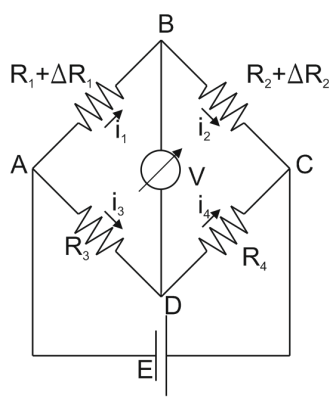
\includegraphics[width=0.5\linewidth]{immagini/screenshot017}
\end{center}
Posizione finale = \ang{180.000} + \ang{22.500} + \ang{5.6250} + \ang{2.8125}=\ang{210.9375}
\end{adjustwidth}
\newpage
\subsection{Laser a triangolazione}
\begin{adjustwidth}{2in}{}	 
	Il laser a triangolazione è un sistema di misura che avviene senza contatto diretto, con LVDT o potenziometro è sempre necessario collegare l'oggetto della misurazione. 
	\begin{center}
		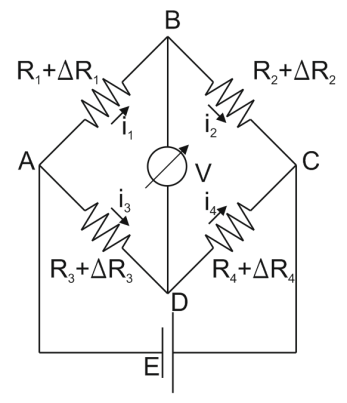
\includegraphics[width=0.3\linewidth]{immagini/screenshot018}
	\end{center}
	Tale laser si basa sull'emissione e sulla ricezione di un segnale ottico: Un diodo proietta la luce nel visibile sulla superficie de target di misura, la luce riflessa da questo target viene nello stesso tempo registrata da un sensore CCD/CMOS. 
	\[\underset{a}{\rightarrow} \boxed{} \underset{\lambda}{\rightarrow}\] 
	\begin{center}
		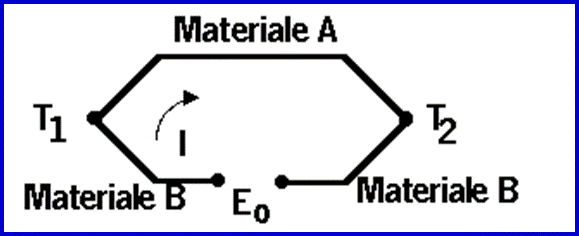
\includegraphics[width=0.5\linewidth]{immagini/screenshot019}
	\end{center}
	In cui 
	\begin{itemize}
		\item a: distanza dallo zero, è la distanza per la quale il raggio riflesso incide centralmente il sensore ottico.
		\item b: campo di misura, indica la zona dove l'oggetto si può muovere, oltre quella distanza la luce riflessa non entra più nel sensore ottico. 
	\end{itemize}
	Un generico laser a triangolazione è caratterizzato dalle seguenti caratteristiche 
	\begin{itemize}
		\item Lunghezza d’onda del laser di \SI{670}{\nano\metre} (rosso)
	\item Ampie distanze fra sensore e target \SI{50}{\milli\metre}$\div$\SI{250}{\milli\metre}
	\item Range di misura da $\pm$\SI{2}{\milli\metre}$\div\pm$\SI{100}{\milli\metre} 
	\item Precisione: 0,005\% FS
	\item Linearità dello 0,03\% FS
	\item Temperatura di funzionamento da \SI{0}{\degreeCelsius} a \SI{40}{\degreeCelsius}
	\end{itemize}
	
	\begin{center}
		\textbf{Se per tutti questi sensori è possibile ottenere una misura di velocità indiretta dalla misura dello spostamento, con i seguenti si potrà risalire ad una misura diretta della velocità.} 
	\end{center}
\end{adjustwidth}
\newpage			
\section{Misure di Velocità}
\subsection{Sistemi ad Induzione Magnetica}
\begin{adjustwidth}{2in}{}
	Questi sistemi si basano sulla legge dell'induzione elettromagnetica
	\[E_0 = Blv\]
	In cui 
	\begin{itemize}
		\item $E_0$ è la tensione generata dal trasduttore 
		\item $B$ è la componente di densità del flusso, normale al vettore di velocità
		\item $l$ è la lunghezza del conduttore 
		\item $v$ è la velocità
	\end{itemize}
	Il vantaggio di questo sistema è che nell'equazione fisica dello strumento compare direttamente la velocità.
	\begin{center}
		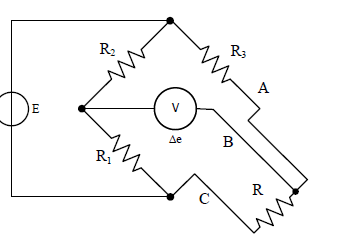
\includegraphics[width=0.5\linewidth]{immagini/screenshot021}
	\end{center}
	Il trasduttore di velocità equivale così ad un generatore di tensione connesso in serie ad un'induttanza $L_T$ e ad una resistenza $R_T$ e collegato ad uno strumento per il rilievo della tensione caratterizzato da una resistenza in ingresso $R_S$. 
	\begin{center}
		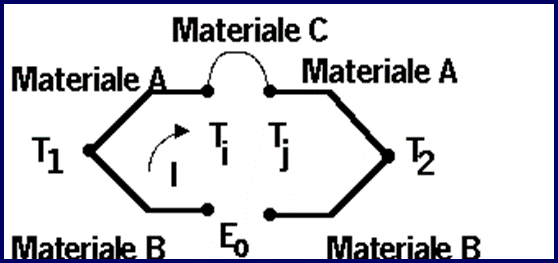
\includegraphics[width=0.5\linewidth]{immagini/screenshot022}
	\end{center}
	\begin{center}
		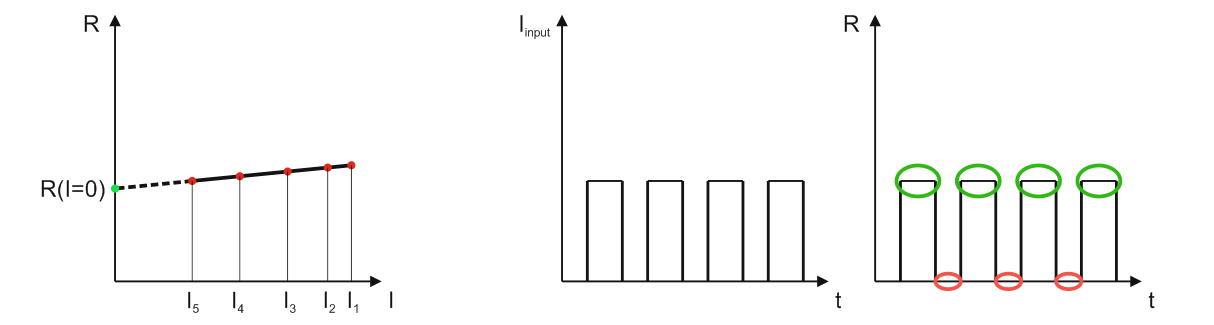
\includegraphics[width=0.5\linewidth]{immagini/screenshot023}
	\end{center}
	La risposta diviene sempre così in funzione della frequenza del segnale in ingresso. 
	\[L_r\dfrac{di(t)}{dt} + (R_r+R_s)i(t) = E_0=S_vv(t)\]
	In cui
	\[i(t) = Ie^{j\omega t}\qquad v(t)=Ve^{j\omega t}\]
	Portando a 
	\[(R_r+R_s+jL_r\omega)I = S_vV\]
	\[H(j\omega) = \dfrac{I}{V} = \dfrac{S_v}{R_r+R_s+jL_r\omega}\]
	Dove si possono individuare
	\begin{itemize}
		\item \(S_v\) Sensibilità del trasduttore 
		
		\item $v$ velocità istantanea [\si{\metre\per\second}]
		
		\item $I, V$ valori istantanei dell'intensità di corrente e di tensione
	\end{itemize}
	\begin{center}
		\textbf{Importante notare come si possa anche misurare uno spostamento indiretto tramite questi strumenti: basta derivare il segnale.}
	\end{center}
	\newpage
	{\LARGE \textbf{NOTE}}

\end{adjustwidth}
\end{document}